% Measurement pipeline, Fig. 1. Drawn in TikZ so it sets in the paper's own
% Times rather than in a plotting library's sans, and so the rules and the
% body text share a colour. Compile standalone:
%   pdflatex fig_pipeline.tex && mv fig_pipeline.pdf fig_pipeline_compact.pdf
% Geometry is millimetres at the size the figure is printed, width 141mm at
% 0.78\textwidth, so nothing is rescaled on inclusion and 8pt here is 8pt on
% the page. Numbers are literals from main.tex.
\documentclass[border=1pt]{standalone}
\usepackage{times}
\usepackage{tikz}
\usetikzlibrary{arrows.meta}

\definecolor{ink}{gray}{0.10}
\definecolor{note}{gray}{0.20}
\definecolor{rule}{gray}{0.55}

\begin{document}
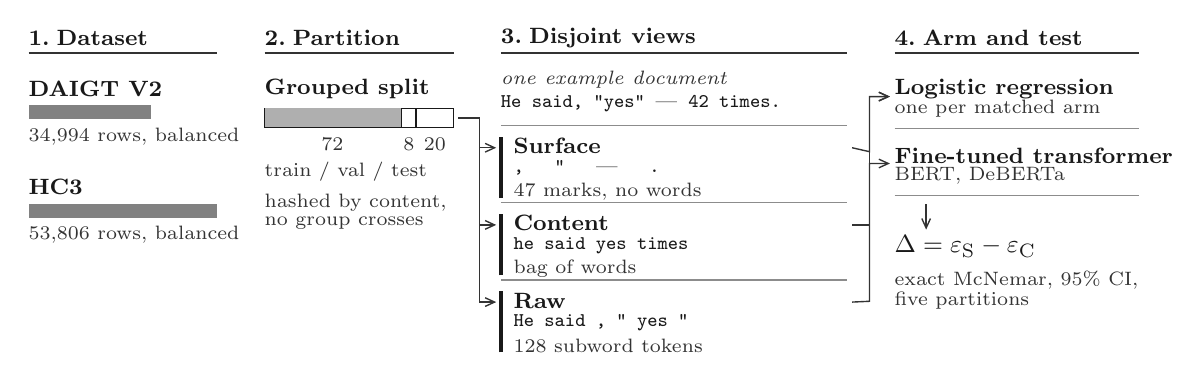
\begin{tikzpicture}[x=1mm,y=1mm,
  every node/.style={inner sep=0pt,outer sep=0pt,text=ink},
  hd/.style={font=\bfseries\fontsize{8.2}{9.4}\selectfont,anchor=west},
  nm/.style={font=\bfseries\fontsize{8}{9}\selectfont,anchor=west},
  nt/.style={font=\fontsize{7.3}{8.4}\selectfont,text=note,anchor=west},
  sp/.style={font=\ttfamily\fontsize{7.3}{8.4}\selectfont,anchor=west},
  eq/.style={font=\fontsize{9.5}{11}\selectfont,anchor=west},
  flow/.style={draw=note,line width=0.5pt,-{Straight Barb[length=1.2mm,width=1.1mm]}}]

% ---- stage headers -------------------------------------------------------
\foreach \x/\w/\n/\t in {0/24/1/Dataset, 30/24/2/Partition,
                         60/44/3/{Disjoint views}, 110/31/4/{Arm and test}} {
  \node[hd] at (\x,44) {\n.\hspace{0.9mm}\t};
  \draw[note,line width=0.6pt] (\x,42) -- (\x+\w,42);
}

% ---- 1  dataset ----------------------------------------------------------
\node[nm] at (0,37.5) {DAIGT V2};
\fill[ink!55] (0,33.6) rectangle (15.6,35.4);
\node[nt] at (0,31.4) {34,994 rows, balanced};
\node[nm] at (0,25) {HC3};
\fill[ink!55] (0,21.1) rectangle (24,22.9);
\node[nt] at (0,18.9) {53,806 rows, balanced};

% ---- 2  partition --------------------------------------------------------
\node[nm] at (30,37.5) {Grouped split};
\draw[ink,line width=0.55pt] (30,32.6) rectangle (54,35);
\draw[ink,line width=0.55pt] (47.3,32.6) -- (47.3,35);
\draw[ink,line width=0.55pt] (49.2,32.6) -- (49.2,35);
\fill[ink!35] (30,32.6) rectangle (47.3,35);
\node[nt,anchor=center] at (38.6,30.4) {72};
\node[nt,anchor=center] at (48.3,30.4) {8};
\node[nt,anchor=center] at (51.6,30.4) {20};
\node[nt] at (30,27) {train / val / test};
\node[nt] at (30,23) {hashed by content,};
\node[nt] at (30,20.4) {no group crosses};

% ---- 3  disjoint views ---------------------------------------------------
\node[nt,font=\itshape\fontsize{7}{8}\selectfont] at (60,38.6) {one example document};
\node[sp] at (60,35.6) {He said, "yes" \textrm{\textemdash} 42 times.};

\foreach \y/\ttl/\spec/\nte in {%
  29/Surface/{,\ \ \ "\ \ \ \textrm{\textemdash}\ \ \ .}/{47 marks, no words},
  19.2/Content/{he said yes times}/{bag of words},
  9.4/Raw/{He said , " yes "}/{128 subword tokens}} {
  \draw[ink,line width=1.2pt] (60,\y-5.4) -- (60,\y+2.4);
  \node[nm] at (61.6,\y+1.2) {\ttl};
  \node[sp] at (61.6,\y-1.6) {\spec};
  \node[nt] at (61.6,\y-4.6) {\nte};
}
\draw[rule,line width=0.45pt] (60,32.8) -- (104,32.8);
\draw[rule,line width=0.45pt] (60,23) -- (104,23);
\draw[rule,line width=0.45pt] (60,13.2) -- (104,13.2);

% ---- flow, partition to views -------------------------------------------
\foreach \y in {30,20.2,10.4} {
  \draw[flow] (54.6,33.8) -- (57.3,33.8) -- (57.3,\y) -- (59.4,\y);
}

% ---- 4  arm and test -----------------------------------------------------
\node[nm] at (110,37.5) {Logistic regression};
\node[nt] at (110,35) {one per matched arm};
\draw[rule,line width=0.45pt] (110,32.4) -- (141,32.4);
\node[nm] at (110,29) {Fine-tuned transformer};
\node[nt] at (110,26.5) {BERT, DeBERTa};
\draw[rule,line width=0.45pt] (110,23.9) -- (141,23.9);
\node[eq] at (110,17.5) {$\Delta=\varepsilon_{\mathrm{S}}-\varepsilon_{\mathrm{C}}$};
\node[nt] at (110,13.2) {exact McNemar, 95\% CI,};
\node[nt] at (110,10.6) {five partitions};

\draw[flow] (104.6,30) -- (106.8,29.5) -- (106.8,36.5) -- (109.4,36.5);
\draw[flow] (104.6,20.2) -- (106.8,20.2) -- (106.8,36.5) -- (109.4,36.5);
\draw[flow] (104.6,10.4) -- (106.8,10.5) -- (106.8,28) -- (109.4,28);
\draw[flow] (114,22.8) -- (114,19.6);
\end{tikzpicture}
\end{document}
